\documentclass{beamer}
\usepackage[spanish]{babel}
\usepackage[latin1]{inputenc}
\usetheme{Warsaw}
\useoutertheme{shadow}


\begin{document}

\begin{frame}
    \frametitle{BrainStorm optimization}
    \begin{figure}
		\centering
		
\includegraphics[width=0.7\linewidth]{blog_brainstorming}
		\label{fig:blog_brainstorming}
	\end{figure}

\end{frame}

\begin{frame}
	\frametitle{Brainstorm optimization}
	Se basa en el comportamiento humano para resolver problemas.
	\begin{itemize}
		\item \textbf{Generar primeras ideas sin prejuicios} 
		\item \textbf{Agrupar ideas parecidas}
		\item \textbf{Fusionar ideas prometedoras pero de distintos grupos}
		\item \textbf{Intentar mejorar buenas ideas.}
	\end{itemize}
\end{frame}

\begin{frame}
	\frametitle{Brainstorm optimization}
	\textbf{Generaci�n de ideas}
	
	\begin{figure}
		\centering
		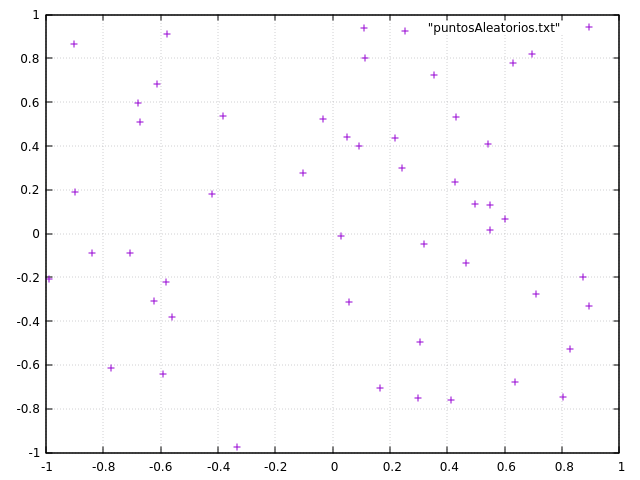
\includegraphics[width=0.7\linewidth]{PrimerasIdeas}
		\label{fig:PrimerasIdeas}
	\end{figure}

\end{frame}

\begin{frame}
	\frametitle{Brainstorm optimization. Clustering.}
	\begin{figure}
		\centering
		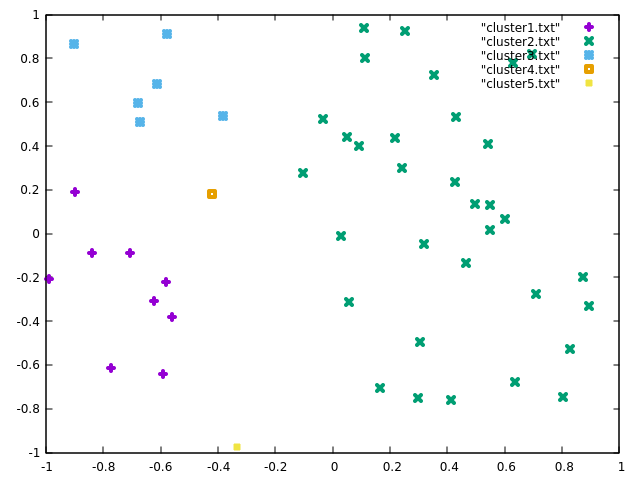
\includegraphics[width=0.7\linewidth]{clusterIdeas}
		\label{fig:clusterIdeas}
	\end{figure}

\end{frame}

\begin{frame}
	\frametitle{Brainstorm optimization. Clustering.}
	En el paper no se realiza ninguna propuesta. Aqu� algunos m�todos de clustering:\\
	\begin{itemize}
		\item Clustering por cercan�a.
		\item Clustering por centroide.
		\item Distribuci�n, densidad...
	\end{itemize}
	En el ejemplo hemos utilizado el primer tipo, siendo la funci�n de distancia de un cluster a otro:\\
	
	\[d(C1,C2) = min\{d(x,y):x	\in C1, y \in C2 \}\]
\end{frame}

\begin{frame}
	\frametitle{Brainstorm optimization. Selecci�n de centros de clusters.}
	
	\[coste(x) = \sum \left| cos(x_i) \right| \]
	\begin{figure}
		\centering
		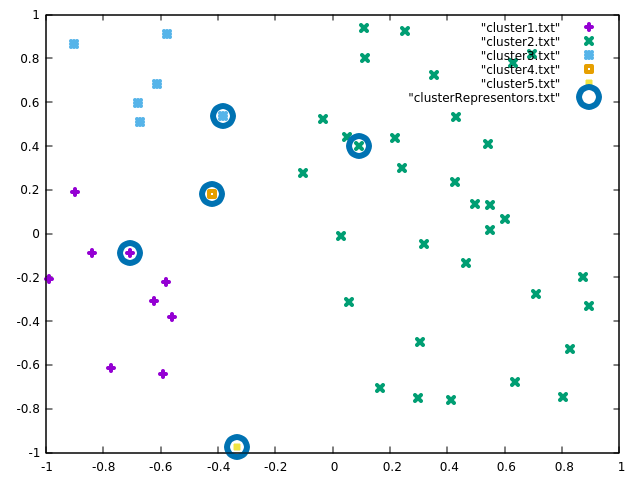
\includegraphics[width=0.7\linewidth]{representantesCluster}
		\label{fig:representantesCluster}
	\end{figure}

	
\end{frame}

\begin{frame}
	\frametitle{Brainstorm optimization}
	\begin{itemize}
		\item \textbf{Posible mutaci�n de alguna idea.}
		
		\begin{itemize}
			\item  \[X^d_{new} <-X^d_{selected} + \psi \times n(0,1) \]
		
			\item \[\psi = logsig\left(\dfrac{\dfrac{Max_{iter}}{2}-Curr_{iter}}{k}\right)\times random()\]
		\end{itemize}
		
	\end{itemize}
		
	
\end{frame}

\begin{frame}
	\frametitle{Brainstorm optimization:par�metros de modificaci�n}
	\textbf{Funci�n sigmoide.}
	\begin{figure}
	\centering
	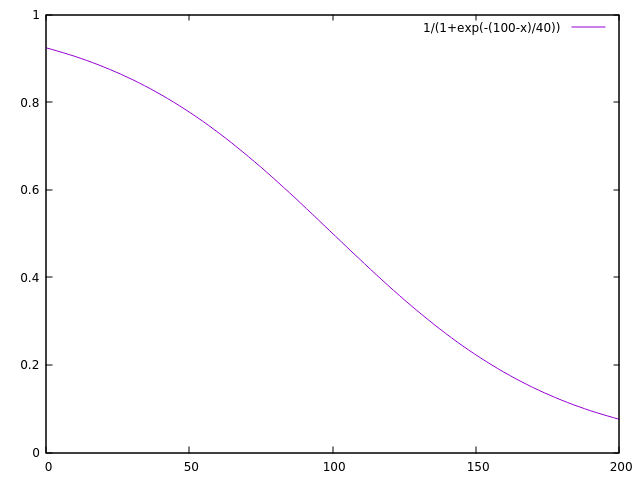
\includegraphics[width=0.4\linewidth]{logsig.png}
	\label{fig:logsig}
	\end{figure}
	
	\textbf{Normal (0,1) }
	\begin{figure}
		\centering
		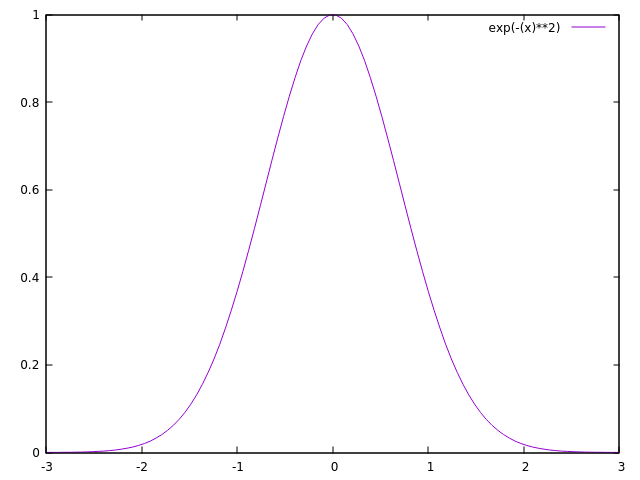
\includegraphics[width=0.4\linewidth]{normal.png}
		\label{fig:normal}
	\end{figure}
	
\end{frame}

\begin{frame}
	\frametitle{Brainstorm optimization. Combinaci�n de ideas prometedoras.}
	
	Ninguna propuesta en el paper, pero:
	
	\begin{itemize}
		\item $X_{new} = \dfrac{X_1+X_2}{2}$ (Media aritm�tica)
		\item $X_{new} = X_1 + F\times(X_2-X_3)$ (Recombinaci�n diferencial)
	\end{itemize}
	
\end{frame}

\begin{frame}
	\frametitle{Brainstorm optimization. Procedimiento.}
	\textbf{�C�mo se escogen las ideas a modificar?}
	\begin{itemize}
		\item Los centros de cluster suelen ser la mejor opci�n para modificar, aunque se debe diversificar la b�squeda con las ideas del mismo cluster.
		\item Podemos alcanzar ideas mejores a partir de explorar una idea buena o recombinando varias ideas buenas(aleatoriamente).
		\item Los clusters con m�s ideas se  modificar�n con m�s frecuencia.
		\item Nos quedaremos con los individuos que mejoren a su idea predecesora.(Posible mejora?).
	\end{itemize}
\end{frame}

\begin{frame}
	\frametitle{Brainstorm optimization.}
	
	Ejemplo de ejecuci�n en 2 dimensiones para Rastrigin.
	
\end{frame}

\begin{frame}
	\frametitle{Brainstorm optimization. Selecci�n de par�metros.}
	
	\begin{array}{|l|l|l|l|l|l|}
		\hline
		n & m & p_{mutaci�n}& p_{explotaci�n} & p_{clusterCenter} & p_{comb. Centros} \\ \hline
		100 & 5 & 0.2 & 0.8 & 0.4 & 0.5 \\ \hline
	\end{array} 
	
	\begin{array}{|l|l|l|l|}
		\hline
		k & Max_{iteraciones} & $\mu$ & $\sigma$ \\ \hline
		20 & 2000 & 0 & 1\\ \hline
	\end{array} 
	
 \end{frame}


\begin{frame}
	\frametitle{Brainstorm optimization: Comparaci�n}
	Comparaciones en el paper...
	\begin{itemize}
		\item  \textbf{Sphere:} $f(X)=\sum_{i=0}^{d}X_i^2$
		\item \textbf{Rastrigin:} $f(X)=\sum_{i=0}^{d}(X_i^2-10cos(2\pi X_i)+10)$
	\end{itemize}
	
	\begin{figure}
	\centering
	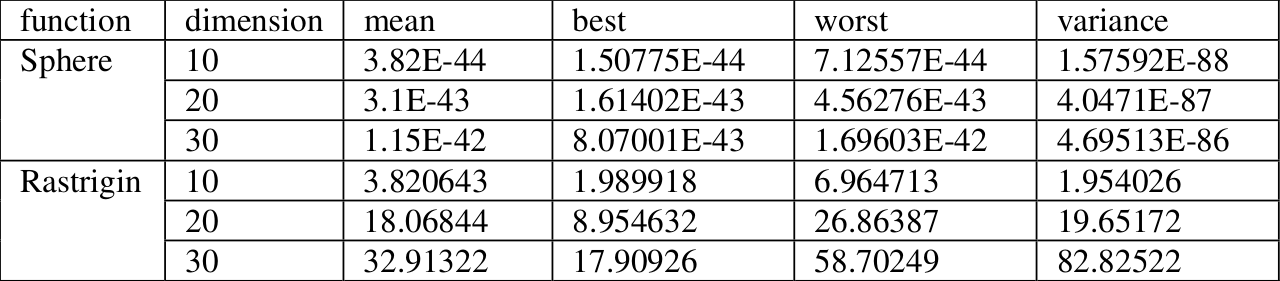
\includegraphics[width=0.9\linewidth]{TablaResultadosPaper}
	\label{fig:TablaResultadosPaper}
	\end{figure}
	
	No hemos obtenido el c�digo, pero las pruebas no lo corroboran(algunas modificaciones realizadas)...
	
	
	
	
\end{frame}

\begin{frame}
	\frametitle{Brainstorm optimization: Posibles mejoras.}
	
	\begin{itemize}
		\item La mutaci�n abusa de la aleatoriedad(N(0,1)*random()).
		\item Aplicar las distintas b�squedas locales a peque�a escala en el proceso de mutaci�n.
		\item Usar distintos m�todos de clustering.
		\item Competici�n de las nuevas ideas con todos sus progenitores.
	\end{itemize}
\end{frame}




\end{document}